\chapter{Gestió de bateries: BMS}
\label{chap:BMS}


Un BMS (Battery Management System) és un sistema electrònic que \newline s'encarrega de gestionar una bateria, des de la càrrega i la descàrrega com el balanceig i el control de la temperatura. Així doncs, ha de poder contemplar certs paràmetres d'una bateria per maximitzar el seu rendiment, mantenir o allargar la seva vida útil, en el nostre cas ens centrarem amb bateries LiPo que són un tipus de bateries amb molta densitat energètica que necessiten disposar d'un BMS.

Un BMS està composat per un hardware i un software que controlen la càrrega i la descàrrega d'una bateria garantint al mateix temps una operació confiable i segura. Això implica el control dels nivells de corrent i tensió, de les condicions de càrrega i descàrrega, de la limitació de la finestra d'operació respecte del SOC i/o la temperatura, de la gestió tèrmica, del balanç en tensió entre les cel·les, etc. Un apropiat sistema de gestió capaç de predir la màxima energia i potència disponible per una connexió i desconnexió segura de les cadenes farà que millorin el seu ús. Un BMS no només controla les funcions d'emmagatzemament per optimitzar la vida útil, eficiència i seguretat del dispositiu, si no que proveeix una precisa estimació dels estats de la bateria per a la gestió energètica. 

\newpage

Els BMS compten amb dos importants enfocaments operacionals, monitoratge i control, que no poden ser separats durant l'operació, per exemple, per garantir un apropiat, ràpid i precís control de la càrrega i descàrrega de les bateries és necessari un sistema de monitoreig que analitzi el voltatge, el corrent, la temperatura interna, SOC i SOH (State of Health), tot protegint la bateria contra situacions perilloses com sobrecàrregues i descàrre- \newline gues profundes.

\begin{figure}[H]
	\centering
    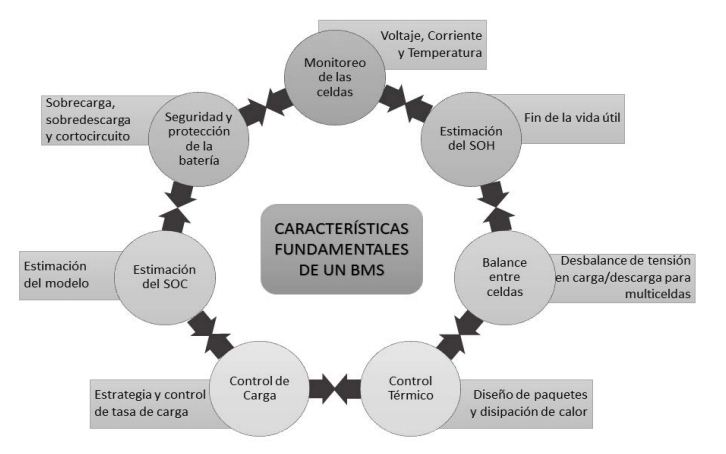
\includegraphics[width=\textwidth, height=10cm] {BMS/diagramabms.png}
    \caption{Característiques fonamentals d'un BMS.}
\end{figure}

\section{Perquè es necessita un BMS?}
El motiu principal de la necessitat d'un gestor de bateries és el fet de que les bateries encara han de millorar molt tecnològicament i han de ser més segures. La majoria de les bateries funcionen prou bé dintre d'uns certs marges, fóra d'aquests la bateria perilla. El problema principal de les bateries de liti és que són molt intolerants a sobrecàrregues i descàrregues profundes, si aquestes coses no es protegeixen no només perilla la bateria, sinó que si la bateria està instal·lada dins d'un vehicle i explota podria provocar greus conseqüències. És per això que si un òptim BMS que controli les condicions operacionals de la bateria per a prolongar la seva vida útil i garanteixi la seva seguretat a través de l'estimació dels paràmetres SOC i SOH, és molt important. 
Tot això és possible gràcies a que el BMS posseeix característiques per al control i monitoreig de l'estat de cada cel·la i així conèixer el seu estat actual, predir la seva capacitat i controlar l'intercanvi energètic. Encara aquí la precisió en l'estimació juga un paper fonamental, fins al punt de convertir-se en un factor normatiu que posseeix diferents conflictes: precisió dels sensors i sistemes d'adquisició de dades, necessitat d'arribar a un objectiu tècnic donat, esforç degut al rendiment de la bateria, qualitat dels models i algorismes emprats. Per tant, una confiable estimació del SOC i SOH no només és \newline  necessària contra descàrregues profundes o sobrecàrregues, prolonga la vida de la bateria i la prediu.  

És vital que tot BMS porti sensors de temperatura per a monitorar en tot moment les cel·les. Ja sabem que les bateries de liti tenen un alt risc si es surten dels límits que permet el fabricant. És per això que cal controlar la temperatura de les cel·les per tractar d'evitar que es puguin arribar a encendre i que malmetin el BMS. Si per exemple una cel·la d'una bateria està carregant-se per sobre del seu voltatge, aquesta comença a augmentar la seva temperatura ja que hi està circulant més corrent. Si no s'aplica cap mesura, la cel·la pot arribar a incendiar-se, provocant inclús danys a les altres cel·les i, en el pitjor dels casos, cremar tota la bateria o explotar. Això comporta que s'estableixin unes certes mesures de seguretat i no hi ha millor opció que el BMS. En el fons s'encarrega de protegir les bateries i protegir a l'individu que estigui manipulant-les.

\section{Quins elements té en compte un BMS?}
Un BMS pot controlar l'estat de la bateria tal com es representen diversos elements, com ara:
\begin{itemize}	
	\item Voltatge: tensió total, voltatges de cel·les individuals, tensió mínima o màxima de cel·les o tensió de taps periòdics.
    \item Temperatura: temperatura mitjana, temperatura d'entrada de refrigerant, temperatura de sortida del refrigerant o temperatures de cel·les individuals.
    \item Estat de càrrega (SOC) o profunditat de descàrrega (DOD), per indicar el nivell de càrrega de la bateria.
    \item Estat de salut (SOH), una mesura diferentment definida de la capacitat restant de la bateria com a percentatge de la capacitat original.
    \item Estat de potència (SOP), la quantitat de potència disponible per a un interval de temps definit, tenint en compte el consum d'energia actual, la temperatura i altres condicions.
    \item Fluid refrigerant: per a bateries d'aire o de refrigeració fluida.
    \item Corrent : actual dins o fora de la bateria. 
    \item frenada regenerativa: controlarà la recàrrega de la bateria redirigint l'energia recuperada de tornada al paquet de bateria.
    \item Corrent màxim de càrrega com a límit de corrent de càrrega.
    \item Corrent de càrrega màxim com a límit de corrent de descàrrega.
	\item Energia [kWh] lliurada des de l'última càrrega o cicle de càrrega.
	\item Impedància interna d'una cel·la (per determinar la tensió del circuit obert).
	\item Càrrega [Ah] lliurada o emmagatzemada (de vegades aquesta característica es diu comptador Coulomb).
	\item Energia total lliurada des del primer ús.
	\item Temps total de funcionament des del primer ús.
	\item Nombre total de cicles.
    \item Eliminant energia de les cel·les més carregades connectant-les a una càrrega (com mitjançant reguladors passius).
\end{itemize}

\section{Quins càlculs realitza un BMS?}
Un BMS pot calcular valors basats en els ítems d’abaix, com:
\begin{itemize}
	\item Corrent de càrrega màxim com a límit de carrega de corrent (CCL charge current limit).
	\item Corrent de descàrrega com a límit de descarrega de corrent (DCL discharge current limit).
	\item Energia (KWh) entregada des de l’última càrrega o cicles de càrrega.
	\item Impedància interna d’una cel·la (per determinar el voltatge en circuit obert).
	\item Càrrega (Ah) entregada o emmagatzemada (a vegades aquesta característica és nombrada comptador Coulomb).
	\item Energia total entregada des del primer ús.
	\item Nombre total de cicles.
\end{itemize}

Hi ha una gran llista de funcions que pot arribar a desenvolupar el BMS, amb l'actual electrònica i gràcies als microcontroladors és possible arribar a monitoritzar tots aquests paràmetres. No obstant, no es requereixen tenir tots aquests paràmetres per a donar un bon ús a les nostres bateries. El paràmetre que més ens interessa com a usuaris és el SOC. Amb l'estimació del SOC ja s'engloben els voltatges, temperatures i corrents. 

El SOC és l'estat de càrrega, expressat com un percentatge del total de la capacitat màxima que té. Normalment les bateries estan composades per un compost de cel·les. De la mateixa manera que es vol saber l'estat de la bateria, el BMS pot calcular l'estat de cada una de les cel·les i en funció del resultat, descarregar o carregar aquella cel·la més o menys per estabilitzar totes les cel·les de la bateria. El SOC ens permet conèixer en tot moment l'estat de les cel·les.

\section{Estat de càrrega (SOC)}
L'estimació de l'estat de càrrega és essencial per assolir el comportament òptim d'un sistema que controli vehicles elèctrics, ja que el que es vol és poder maximitzar l'utilització del motor elèctric respecte al de combustió.

L'estat de càrrega (SOC) d'una bateria o una cel·la correspon al percentatge de la seva capacitat total d'energia que encara es troba disponible en un determinat moment. No existeix una manera directa de mesurar el SOC d'una bateria degut a l'edat, el voltatge de càrrega, temperatura, velocitat de descàrrega entre altres que afecten la mesura del SOC. El desenvolupament d'una mesura de l'estat de càrrega és un procés molt complex, per la qual es defineix usualment com una estimació en lloc d'una mesura o determinació com a tal. No hi ha un únic procés adequat per a mesurar el SOC.

Un dels factors més importants que afecten a l'estimació del SOC d'una bateria és l'envelliment. Degut als cicles de càrrega i descàrrega, la capacitat de les cel·les que formen la bateria decreix amb el temps. Aquest fet indueix a actualitzar el màxim estat de càrrega disponible per a la bateria periòdicament ja que és la referència per calcular el percentatge abans mencionat. En cas de prendre com a referència el valor nominal per a la capacitat de la bateria, l'estimació pot contenir errors de pes. El procés electroquímic dins de les cel·les al carregar-se i descarregar-se sempre pren un temps finit i no sempre és menor que l'estímul elèctric que càrrega la bateria. Durant el procés de càrrega pot donar-se un pols de descàrrega i no ser realitzat per complert donant lloc a imprecisions en l'estimació del SOC. A més a més, els processos tant de càrrega com descàrrega consumeixen energia i l'energia subministradora per la bateria serà menor que l'utilitzada per a carregar-les. Aquesta proporció rep el nom d'eficiència de Coulomb i pot afectar fins a un 3\% de la capacitat disponible. 

El SOC s'entén com la quantitat de càrrega encara disponible en relació amb la capacitat de la bateria. L'estat de càrrega es calcula amb la relació entre la diferència de la capacitat nominal de la cel·la i la capacitat restant per un costat i la capacitat nominal per l'altre. L'estat de càrrega és 1 quan s'arriba a l'estat complert de càrrega i 0 després d'una descàrrega complerta.

\begin{figure}[H]
	\centering
    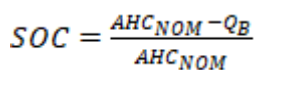
\includegraphics[width=5cm, height=3cm] {BMS/Coulombcountingformula.png}
    \caption{Fórmula elemental per al càlcul del SOC.}
\end{figure}

\begin{itemize}
    \item SOC: Estat de la càrrega de la bateria.
    \item Qb: Càrrega restant.
    \item AHCnom: Capacitat nominal (Hora - Ampere).
\end{itemize}

Abans de parlar dels mètodes més comuns per fer l'estimació del SOC d'una bateria, cal parlar d'un concepte clau en el món de les bateries i el SOC. Aquest concepte és l'histèresi. L'histèresi és la tendència d'un material a conservar les seves propietats. Les bateries estan composades per materials ferromagnètics els quals també tenen una tendència a conserver les seves propietats. En el cas de les bateries i parlant ja en els termes del BMS vindria a ser l'evolució del voltatge en el temps respecte les característiques del material de la cel·la. Com ja hem comentat prèviament dues bateries amb les mateixes característiques tècniques sobre una mateixa càrrega no es descarreguen igual.

És per això que la bateria pot estar a un mateix voltatge però a diferent capacitat. Per tant existeix un rang en el que no podem assegurar únicament amb el voltatge la capacitat. És per això que s'inclouen més variables a l'algorisme per tal d'afinar molt més el SOC.

\begin{figure}[H]
	\centering
    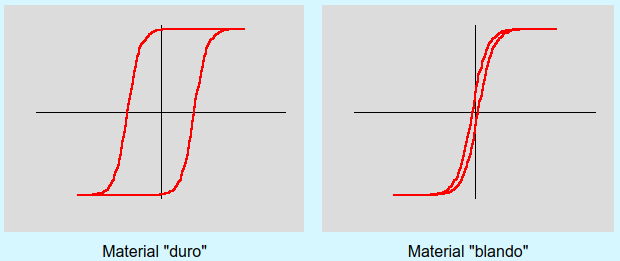
\includegraphics[width=\textwidth, height=7cm] {BMS/histeresis.png}
    \caption{Cicle d'histèresi en funció del material.}
\end{figure}

\subsection{Mètodes d'estimació per al SOC}
Existeixen diferents mètodes per a fer l'estimació del SOC. Els més comuns són els següents:

\begin{itemize}
    \item Mesura directa: Es tracta d'un mètode teòric i hipotètic ja que es basa en la hipòtesi d'un corrent de descàrrega constant. Aquest valor es multiplicat pel temps de descàrrega total de la bateria obtenint-se la capacitat de la pila de bateries. Com es fàcil d'intuir, es tracta d'un mètode inviable ja que el corrent de descàrrega és variable a la pràctica i, a més a més, els usuaris han de conèixer l'estimació del SOC sense descarregar la bateria o, al menys, abans de la descàrrega total de la mateixa.
   
    \item Mesura de la gravetat específica: També és conegut com a mesura de la densitat relativa i és necessari tenir accés a l'electròlit líquid intern de la bateria. Existeix una relació matemàtica entre la densitat de l'aigua i la d'una substància electròlit descendent linealment amb la descàrrega de la cel·la de bateria. Per tant, mesurant la densitat de l'electròlit s'obté una estimació del SOC de la cel·la. Encara que es tracta d'un mètode bastant precís, no és capaç de determinar la capacitat total de la bateria. 
   
    \item Impedància interna: Amb els cicles de càrrega i descàrrega, la composició dels components químics interns a una cel·la canvien i això deriva en una variació de la impedància interna. Aquest paràmetre també és un indicatiu del SOC però la seva mesura pot ser molt difícil durant el funcionament real d'una bateria i, a més a més, té una gran dependència amb la temperatura.
   
    \item Estimació basada en voltatge: Aquest mètode es basa en una relació directa entre el voltatge actual de la bateria i la capacitat disponible de la mateixa. Es tracta d'un mètode poc precís degut al comportament no lineal de molts tipus de bateries amb respecte el voltatge com les d'ió liti. Es pot observar una caiguda abrupta de la tensió a prop de la imminent descàrrega total de la bateria, el qual suposa una situació crítica per la gran majoria de les aplicacions electròniques mòbils. Aquestes característiques fan de la mesura basada en voltatge un bon mètode per estimar els moments de càrrega total i de \newline descàrrega imminent però no per a valors intermedis.
   
    \item Estimació basada en intensitat: També coneguda com Coulomb \newline Counting. Consisteix en la integració del corrent entrant i sortint en la bateria. Bàsicament, aquest mètode integra en el temps la intensitat que carrega i descarrega les cel·les i el seu resultat es la càrrega emmagatzemada en l'interior de les mateixes. És qualificat com el mètode més precís per l'estimació del SOC degut a la mesura directa de la càrrega fluint cap i des de la bateria. No obstant, aquest mètode necessita ser combinat amb algun mètode d'estimació de les condicions de mesura com per exemple el moment d'inici del procés de càrrega. Aquesta estimació és la més emprada en ordinadors, equips mèdics i altres dispositius portàtil.
\end{itemize}  

\section{Control de la temperatura}
Com ja s'ha anat esmentat al llarg del projecte, les bateries han de poder funcionar dintre d'un rang de temperatures. Fora d'aquest rang, tant la bateria com l'usuari pot sofrir danys. Sortir dels rangs de temperatura de funcionament que indica el fabricant és un dels majors errors que es pot cometre quan es manipula una bateria.

El control de la temperatura no es té en compte únicament per a que miri que les cel·les no surtin dels rangs. També es té en compte quan la bateria es troba dintre dels seus rangs de treball. La diferència de temperatura entre cel·les dintre dels rangs òptims de treball d'aquestes, també ens dóna informació profitosa. Normalment la cel·la més calenta, serà la que estigui més carregada i/o bé que hi estigui passant el major corrent. És per això que calcular de forma periòdica la temperatura ajuda al càlcul de l'estat de la cel·la, i per tant, del SOC. Com ja s'ha comentat en el punt anterior l'estimació del SOC ens dóna la idea de la capacitat actual de la cel·la. Si no es tingués en compte la temperatura, l'estimació seria molt menys precisa. A més a més, és una variable vital de monitoreig per a prediccions de futur en aplicacions molt complexes.

La temperatura és l'indicatiu més pròxim que ens indica si la bateria es troba en un estat de risc o no. Pot ser que a dins d'una bateria, les cel·les no estiguin correctament balancejades i per tant hi hagin problemes de capacitat a la bateria. El fet de que no estiguin balancejades no vol dir que el BMS s'hagi de parar, simplement ha de balancejar. Òbviament si es surten de les condicions de funcionament de les cel·les es provocaria una parada per part del BMS, però només en casos on és exagerat el desbalanceig. En canvi, per a qualsevol detecció de sobre temperatura o sota temperatura és necessari fer una parada forçosa del BMS ja que hi està havent un problema. 

En resum el control de la temperatura és totalment necessari i el fet de no tenir-la en compte ja fa que surti del concepte de BMS.

\newpage

\section{Balanceig entre cel·les}
El balanceig és una de les funcions principals que ha de realitzar el BMS. Més enllà d'actuar com protecció en condicions inadequades per a la bateria de manera que s'eviti el danyar les cel·les, una bona gestió del balanceig permetrà completar els cicles de càrrega i descàrrega òptimament de mode que s'aprofiti la capacitat energètica disponible en la bateria.

\begin{figure}[H]
	\centering
    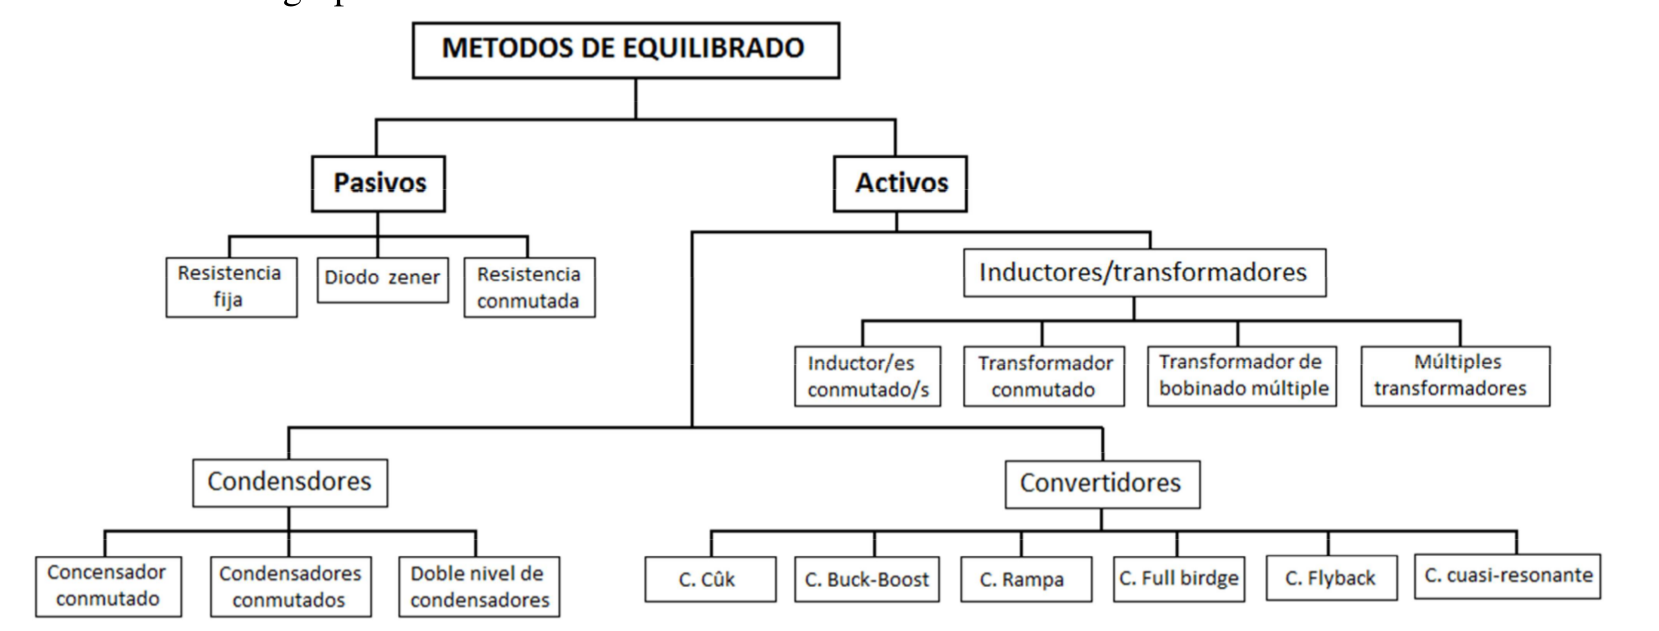
\includegraphics[width=\textwidth, height=12cm] {BMS/metodosequilibrado.png}
    \caption{Mètodes de balanceig de cel·les.}
\end{figure}

\subsection{Causes del desbalanceig de cel·les}
Les principals causes del desbalanceig a les cel·les queden indicades en els següents punts:

\begin{itemize}
    \item Quan es fa el muntatge d'una bateria amb cel·les a diferents nivells de càrrega.
    
    \item Quan es munten cel·les amb el mateix estat de càrrega però diferent historial de cicle. En aquest cas, si bé el sistema d'entrada està balancejat, el desbalanceig començarà a fer-se evident de forma ràpida. El major problema d'aquest desbalanceig es que més enllà de poder-se corregir mitjançant gestions del BMS, tornarà a aparèixer en quan es realitzin cicles ràpids de càrrega i descàrrega. A la pràctica, \newline l'emprar cel·les idèntiques amb diferent ciclat té un efecte similar a posar cel·les amb diferent capacitat. Les cel·les perden capacitat de càrrega/descàrrega conforme són ciclades. Això es per tant un factor que s'ha d'evitar.
    
    \item Per les pròpies diferències entre cel·les producte de toleràncies en la fabricació. Aquestes diferències són causa de petites desviacions de la capacitat real respecte el disseny, de diferents corrents d'auto descàrrega, etc. Aquest és el cas més comú de desbalanceig. Les petites diferències de funcionament entre cel·les es podrà compensar amb l'algorisme de balanceig del BMS de mode que a la pràctica no s'haurien de veure problemes greus de desbalanceig. Com a molt s'ha d'optar per fabricants que garanteixin desviacions petites en el comportament de les cel·les per així eludir part del problema.
    
    \item En molts casos, és el propi BMS el que provoca efectes de desbalanceig. Principalment en bateries amb un nombre de cel·les per sobre de 3, es solen emprar esgraons d'alimentació de mode que grups de cel·les alimenten parts de l'electrònica, i així demanar de forma equivalent a cada cel·La. A la realitat el que succeeix és que hi ha cel·les que contribueixen més a l'alimentació de control que altres i això a llarg plaç podria ser causa d'un desbalanceig de cel·les. El sistema de gestió de balanceig ha de ser capaç de contrarestar aquest efecte, que a més a més, és a molt llarg plaç doncs els consums dels sistemes de gestió śon de molt poca potència.
\end{itemize}

\subsection{Balanceig passiu}
És el balanceig més emprat. Es basa en descarregar la cel·la o cel·les més carregades mitjançant una resistència. Aquesta tècnica empra una \newline resistència per dissipar l'excés de càrrega que pot acumular una cel·la fins que la seva tensió de sortida cau per sota del punt de voltatge de regulació. És per això que també reben el nom de balanceig dissipatiu. Els grans avantatges del mode passiu són el baix cost de components i la simplicitat en el disseny i control. Òbviament, el gran inconvenient és que tota l'energia manejada en el procés de balanceig és una energia perduda.

L'algorisme bàsic es pot fer més complex tenint en compte altres variables de decisió com pot ser la tensió de cel·la o el mode en el que es trobi la bateria. Per un costat, és convenient establir una tensió mínima de cel·la per la qual la gestió de balanceig es desactivi. Això garanteix que en sistemes amb baix estat de càrrega de les cel·les, el balanceig les descarregui encara més.

Una altra configuració habitual és permetre el balanceig només quan la bateria es troba en mode càrrega. Imaginem la bateria amb un estat de càrrega X, i es deixa durant setmanes o mesos sense ús. Si el balanceig actua, pot provocar que l'estat de carrega real al cap de les setmanes sigui molt diferent al que indica la bateria. Per altra banda, en un procés de carrega complert es produeix l'actualització de l'estat de càrrega del sistema, amb el qual no afecta en aquest aspecte el tenir activat el balanceig.

\begin{figure}[H]
	\centering
    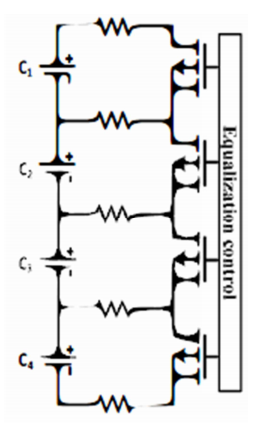
\includegraphics[width=7cm, height=7cm] {BMS/balanceopasivoresistcomutada.png}
    \caption{Balanceig passiu per resistència commutada}
\end{figure}

El dimensionat del circuit de balanceig es basa en decidir el corrent màxim de balanceig. Aquest valor ha de ser un compromís entre diferents aspectes. Per un costat, interessaran corrents alts de mode que un possible desbalanceig sigui corregit el més ràpid possible per part del BMS. Pel contrari, sobredimensionar aquest circuit implica utilitzar transistors mosfets i resistències de major potència, amb el que això suposa un cost de components així com espai per a l'electrònica.

\subsection{Balanceig actiu}
El balanceig actiu de les cel·les d'una bateria està adquirint cada cop més importància ja que soluciona els principals defectes del balanceig passiu. També presenta els seus propis inconvenients, per a un gran nombre de cel·les pot arribar a resultar una cosa antieconòmica. El principal avantatge d'aquest equilibrat és que no dissipa la càrrega que tenen en excés les cel·les sinó que l'utilitza per equilibrar cel·les menys carregades a través de condensadors o inductors aconseguint un ús més eficient de l'energia i un major compte sobre la bateria, el que augmenta la seva vida útil.

Els principals inconvenients d'aquest tipus de balanceig són:
\begin{itemize}
    \item Complexitat i cost de l'electrònica associada al balanceig.
    \item Complicació en la gestió del balanceig.
    \item Sorolls de commutació.
\end{itemize}

El mètode principal en la majoria d'implementacions de BMS amb balanceig actiu es realitza mitjançant una càrrega capacitiva. És a dir, fent servir un condensador.

Aquest mètode es basa en curtcircuitar la cel·la més carregada a un condensador i a continuació buidar aquest sobre la cel·la adjacent més descarregada. Aquest mètode té moltes limitacions.

Per una banda l'electrònica de commutació ha de poder manejar els pics de corrent que es produiran en els processos de càrrega i descàrrega. Les pèrdues d'energia poden estar al voltant del 50\%. Un altre problema és que la capacitat de transferència d'energia és proporcional a la diferència de tensions entre les cel·les de càrrega i descàrrega amb lo que el balanceig serà efectiu només en els extrems dels cicles de càrrega per ser les zones on es donaran les majors diferències de tensió entre cel·les. Aquests pics de corrent a més a més provocaran soroll en l'electrònica de control que ha de ser tingut molt en compte per evitar problemes en les mesures.

El balanceig es farà lent a mesura que hi hagi més cel·les en sèrie. Si es suposa que hi ha 3 cel·les en sèrie, sent la cel·la 1 la més carregada i la cel·la 3 la més descarregada. Idealment el balanceig actiu per càrrega capacitiva hauria de carregar el condensador amb la cel·la 1 i descarregar-ho a la 3, però com no són cel·les adjacents primerament es tindrà que transferir potència de la 2 a la 3 a menor ritme i després de la 1 a la 2. Si ara en comptes d'haver-hi 3 cel·les tenim 30 i volem descarregar la 10 i transferir-la a la 30, caldrà passar per les 18 cel·les intermèdies i per tant, és un procés lent.

\begin{figure}[H]
	\centering
    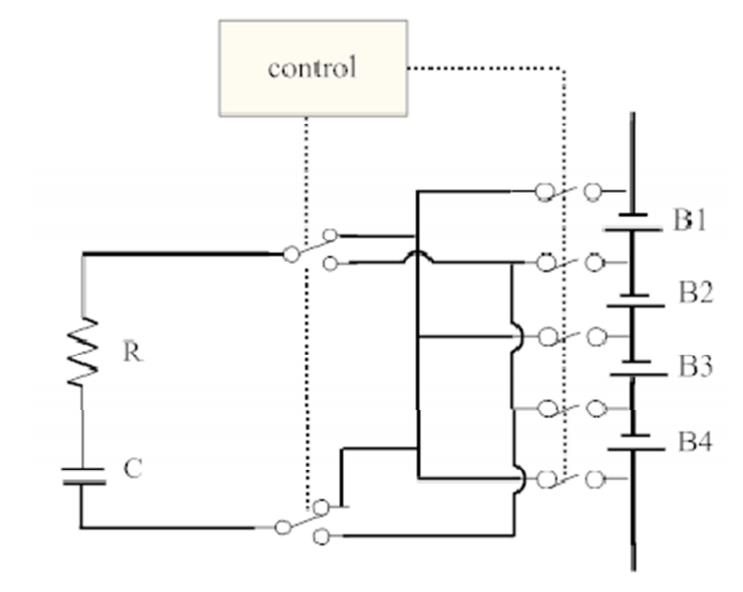
\includegraphics[width=8cm, height=8cm] {BMS/balanceoactivocondensador.png}
    \caption{Balanceig actiu per condensador commutat.}
\end{figure}  

Existeix un segon mètode que està començant a veure's en diferents implementacions del balanceig actiu. Aquest mètode aprofita la càrrega d'una bobina des de la cel·la més carregada per després bolcar l'energia emmagatzemada en aquesta bobina en la cel·la adjacent més descarregada. Millora l'aspecte d'eficiència amb respecte a la càrrega capacitiva principalment pel fet de que els pics de corrent provocats per la topologia capacitiva desapareixen. Això permet a més a més els requeriments en termes de corrent dels components involucrats en el balanceig.

En termes d'eficiència d'operació es pot aconseguir fins a un 90\%. Un altre gran avantatge amb respecte a mode capacitiu és que l'equilibri es pot aconseguir amb independència dels voltatges individuals de les cel·les.

Com aspectes negatius, a més a més d'incrementar els costos i espais dels circuits de balanceig, pot generar problemes de soroll que han de ser tinguts en compte. També, de la mateixa manera que en el cas de balanceig amb càrrega capacitiva, el procés pot alentir-se si hi ha cel·les al mig d'entre les cel·les amb valors de càrrega extrems.

\begin{figure}[H]
	\centering
    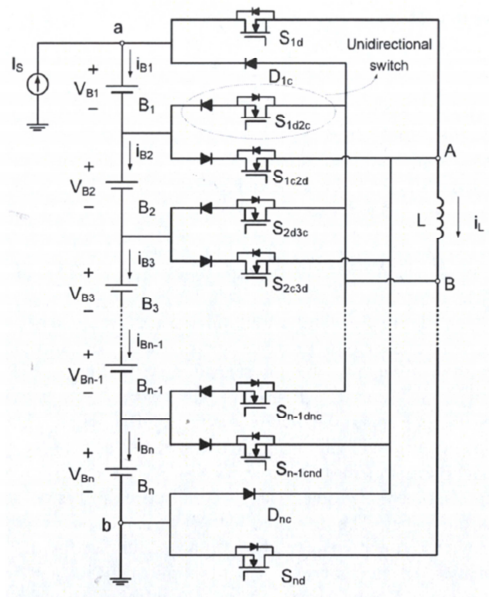
\includegraphics[width=5cm, height=6cm] {BMS/balanceoactivoinductor.png}
    \caption{Balanceig actiu per inductor commutat.}
\end{figure}    

